% Options for packages loaded elsewhere
\PassOptionsToPackage{unicode}{hyperref}
\PassOptionsToPackage{hyphens}{url}
\documentclass[
]{article}
\usepackage{xcolor}
\usepackage[margin=1in]{geometry}
\usepackage{amsmath,amssymb}
\setcounter{secnumdepth}{-\maxdimen} % remove section numbering
\usepackage{iftex}
\ifPDFTeX
  \usepackage[T1]{fontenc}
  \usepackage[utf8]{inputenc}
  \usepackage{textcomp} % provide euro and other symbols
\else % if luatex or xetex
  \usepackage{unicode-math} % this also loads fontspec
  \defaultfontfeatures{Scale=MatchLowercase}
  \defaultfontfeatures[\rmfamily]{Ligatures=TeX,Scale=1}
\fi
\usepackage{lmodern}
\ifPDFTeX\else
  % xetex/luatex font selection
\fi
% Use upquote if available, for straight quotes in verbatim environments
\IfFileExists{upquote.sty}{\usepackage{upquote}}{}
\IfFileExists{microtype.sty}{% use microtype if available
  \usepackage[]{microtype}
  \UseMicrotypeSet[protrusion]{basicmath} % disable protrusion for tt fonts
}{}
\makeatletter
\@ifundefined{KOMAClassName}{% if non-KOMA class
  \IfFileExists{parskip.sty}{%
    \usepackage{parskip}
  }{% else
    \setlength{\parindent}{0pt}
    \setlength{\parskip}{6pt plus 2pt minus 1pt}}
}{% if KOMA class
  \KOMAoptions{parskip=half}}
\makeatother
\usepackage{color}
\usepackage{fancyvrb}
\newcommand{\VerbBar}{|}
\newcommand{\VERB}{\Verb[commandchars=\\\{\}]}
\DefineVerbatimEnvironment{Highlighting}{Verbatim}{commandchars=\\\{\}}
% Add ',fontsize=\small' for more characters per line
\usepackage{framed}
\definecolor{shadecolor}{RGB}{248,248,248}
\newenvironment{Shaded}{\begin{snugshade}}{\end{snugshade}}
\newcommand{\AlertTok}[1]{\textcolor[rgb]{0.94,0.16,0.16}{#1}}
\newcommand{\AnnotationTok}[1]{\textcolor[rgb]{0.56,0.35,0.01}{\textbf{\textit{#1}}}}
\newcommand{\AttributeTok}[1]{\textcolor[rgb]{0.13,0.29,0.53}{#1}}
\newcommand{\BaseNTok}[1]{\textcolor[rgb]{0.00,0.00,0.81}{#1}}
\newcommand{\BuiltInTok}[1]{#1}
\newcommand{\CharTok}[1]{\textcolor[rgb]{0.31,0.60,0.02}{#1}}
\newcommand{\CommentTok}[1]{\textcolor[rgb]{0.56,0.35,0.01}{\textit{#1}}}
\newcommand{\CommentVarTok}[1]{\textcolor[rgb]{0.56,0.35,0.01}{\textbf{\textit{#1}}}}
\newcommand{\ConstantTok}[1]{\textcolor[rgb]{0.56,0.35,0.01}{#1}}
\newcommand{\ControlFlowTok}[1]{\textcolor[rgb]{0.13,0.29,0.53}{\textbf{#1}}}
\newcommand{\DataTypeTok}[1]{\textcolor[rgb]{0.13,0.29,0.53}{#1}}
\newcommand{\DecValTok}[1]{\textcolor[rgb]{0.00,0.00,0.81}{#1}}
\newcommand{\DocumentationTok}[1]{\textcolor[rgb]{0.56,0.35,0.01}{\textbf{\textit{#1}}}}
\newcommand{\ErrorTok}[1]{\textcolor[rgb]{0.64,0.00,0.00}{\textbf{#1}}}
\newcommand{\ExtensionTok}[1]{#1}
\newcommand{\FloatTok}[1]{\textcolor[rgb]{0.00,0.00,0.81}{#1}}
\newcommand{\FunctionTok}[1]{\textcolor[rgb]{0.13,0.29,0.53}{\textbf{#1}}}
\newcommand{\ImportTok}[1]{#1}
\newcommand{\InformationTok}[1]{\textcolor[rgb]{0.56,0.35,0.01}{\textbf{\textit{#1}}}}
\newcommand{\KeywordTok}[1]{\textcolor[rgb]{0.13,0.29,0.53}{\textbf{#1}}}
\newcommand{\NormalTok}[1]{#1}
\newcommand{\OperatorTok}[1]{\textcolor[rgb]{0.81,0.36,0.00}{\textbf{#1}}}
\newcommand{\OtherTok}[1]{\textcolor[rgb]{0.56,0.35,0.01}{#1}}
\newcommand{\PreprocessorTok}[1]{\textcolor[rgb]{0.56,0.35,0.01}{\textit{#1}}}
\newcommand{\RegionMarkerTok}[1]{#1}
\newcommand{\SpecialCharTok}[1]{\textcolor[rgb]{0.81,0.36,0.00}{\textbf{#1}}}
\newcommand{\SpecialStringTok}[1]{\textcolor[rgb]{0.31,0.60,0.02}{#1}}
\newcommand{\StringTok}[1]{\textcolor[rgb]{0.31,0.60,0.02}{#1}}
\newcommand{\VariableTok}[1]{\textcolor[rgb]{0.00,0.00,0.00}{#1}}
\newcommand{\VerbatimStringTok}[1]{\textcolor[rgb]{0.31,0.60,0.02}{#1}}
\newcommand{\WarningTok}[1]{\textcolor[rgb]{0.56,0.35,0.01}{\textbf{\textit{#1}}}}
\usepackage{graphicx}
\makeatletter
\newsavebox\pandoc@box
\newcommand*\pandocbounded[1]{% scales image to fit in text height/width
  \sbox\pandoc@box{#1}%
  \Gscale@div\@tempa{\textheight}{\dimexpr\ht\pandoc@box+\dp\pandoc@box\relax}%
  \Gscale@div\@tempb{\linewidth}{\wd\pandoc@box}%
  \ifdim\@tempb\p@<\@tempa\p@\let\@tempa\@tempb\fi% select the smaller of both
  \ifdim\@tempa\p@<\p@\scalebox{\@tempa}{\usebox\pandoc@box}%
  \else\usebox{\pandoc@box}%
  \fi%
}
% Set default figure placement to htbp
\def\fps@figure{htbp}
\makeatother
\setlength{\emergencystretch}{3em} % prevent overfull lines
\providecommand{\tightlist}{%
  \setlength{\itemsep}{0pt}\setlength{\parskip}{0pt}}
\usepackage{bookmark}
\IfFileExists{xurl.sty}{\usepackage{xurl}}{} % add URL line breaks if available
\urlstyle{same}
\hypersetup{
  pdftitle={Class 10: Structural Bioinformatics 1},
  pdfauthor={Yane Lee PID A17670350},
  hidelinks,
  pdfcreator={LaTeX via pandoc}}

\title{Class 10: Structural Bioinformatics 1}
\author{Yane Lee PID A17670350}
\date{2026-02-05}

\begin{document}
\maketitle

\subsection{PDB Statistics}\label{pdb-statistics}

The Protein Data Bank (PDB) is the main repository of biomolecular
strucutres. Let's see what it contains:

\begin{Shaded}
\begin{Highlighting}[]
\NormalTok{stats }\OtherTok{\textless{}{-}} \FunctionTok{read.csv}\NormalTok{(}\StringTok{"Data Export Summary.csv"}\NormalTok{)}
\NormalTok{stats}
\end{Highlighting}
\end{Shaded}

\begin{verbatim}
##            Molecular.Type   X.ray     EM    NMR Integrative Multiple.methods
## 1          Protein (only) 178,795 21,825 12,773         343              226
## 2 Protein/Oligosaccharide  10,363  3,564     34           8               11
## 3              Protein/NA   9,106  6,335    287          24                7
## 4     Nucleic acid (only)   3,132    221  1,566           3               15
## 5                   Other     175     25     33           4                0
## 6  Oligosaccharide (only)      11      0      6           0                1
##   Neutron Other   Total
## 1      84    32 214,078
## 2       1     0  13,981
## 3       0     0  15,759
## 4       3     1   4,941
## 5       0     0     237
## 6       0     4      22
\end{verbatim}

\begin{Shaded}
\begin{Highlighting}[]
\NormalTok{stats}\SpecialCharTok{$}\NormalTok{X.ray}
\end{Highlighting}
\end{Shaded}

\begin{verbatim}
## [1] "178,795" "10,363"  "9,106"   "3,132"   "175"     "11"
\end{verbatim}

\begin{Shaded}
\begin{Highlighting}[]
\FunctionTok{sum}\NormalTok{(stats}\SpecialCharTok{$}\NormalTok{Neutron)}
\end{Highlighting}
\end{Shaded}

\begin{verbatim}
## [1] 88
\end{verbatim}

The comma in these numbers leads to the numbers here bring read as
character.

\begin{Shaded}
\begin{Highlighting}[]
\FunctionTok{c}\NormalTok{(}\StringTok{"100"}\NormalTok{, }\StringTok{"10"}\NormalTok{, }\StringTok{"barry"}\NormalTok{)}
\end{Highlighting}
\end{Shaded}

\begin{verbatim}
## [1] "100"   "10"    "barry"
\end{verbatim}

\begin{Shaded}
\begin{Highlighting}[]
\CommentTok{\#install.packages("readr")}
\FunctionTok{library}\NormalTok{(readr)}
\NormalTok{stats }\OtherTok{\textless{}{-}} \FunctionTok{read\_csv}\NormalTok{(}\StringTok{"Data Export Summary.csv"}\NormalTok{)}
\end{Highlighting}
\end{Shaded}

\begin{verbatim}
## Rows: 6 Columns: 9
## -- Column specification --------------------------------------------------------
## Delimiter: ","
## chr (1): Molecular Type
## dbl (4): Integrative, Multiple methods, Neutron, Other
## num (4): X-ray, EM, NMR, Total
## 
## i Use `spec()` to retrieve the full column specification for this data.
## i Specify the column types or set `show_col_types = FALSE` to quiet this message.
\end{verbatim}

\begin{Shaded}
\begin{Highlighting}[]
\NormalTok{stats}
\end{Highlighting}
\end{Shaded}

\begin{verbatim}
## # A tibble: 6 x 9
##   `Molecular Type`    `X-ray`    EM   NMR Integrative `Multiple methods` Neutron
##   <chr>                 <dbl> <dbl> <dbl>       <dbl>              <dbl>   <dbl>
## 1 Protein (only)       178795 21825 12773         343                226      84
## 2 Protein/Oligosacch~   10363  3564    34           8                 11       1
## 3 Protein/NA             9106  6335   287          24                  7       0
## 4 Nucleic acid (only)    3132   221  1566           3                 15       3
## 5 Other                   175    25    33           4                  0       0
## 6 Oligosaccharide (o~      11     0     6           0                  1       0
## # i 2 more variables: Other <dbl>, Total <dbl>
\end{verbatim}

\begin{Shaded}
\begin{Highlighting}[]
\NormalTok{n.xray }\OtherTok{\textless{}{-}} \FunctionTok{sum}\NormalTok{(stats}\SpecialCharTok{$}\StringTok{\textasciigrave{}}\AttributeTok{X{-}ray}\StringTok{\textasciigrave{}}\NormalTok{)}
\CommentTok{\#n.em \textless{}{-} }
\NormalTok{n.total }\OtherTok{\textless{}{-}} \FunctionTok{sum}\NormalTok{(stats}\SpecialCharTok{$}\NormalTok{Total)}

\NormalTok{n.xray}\SpecialCharTok{/}\NormalTok{n.total}
\end{Highlighting}
\end{Shaded}

\begin{verbatim}
## [1] 0.8095077
\end{verbatim}

\begin{quote}
Q1: What percentage of structures in the PDB are solved by X-Ray and
Electron Microscopy.
\end{quote}

\begin{Shaded}
\begin{Highlighting}[]
\NormalTok{n.xray }\OtherTok{\textless{}{-}} \FunctionTok{sum}\NormalTok{(stats}\SpecialCharTok{$}\StringTok{\textasciigrave{}}\AttributeTok{X{-}ray}\StringTok{\textasciigrave{}}\NormalTok{)}
\NormalTok{n.em }\OtherTok{\textless{}{-}} \FunctionTok{sum}\NormalTok{(stats}\SpecialCharTok{$}\StringTok{\textasciigrave{}}\AttributeTok{EM}\StringTok{\textasciigrave{}}\NormalTok{)}
\NormalTok{n.total }\OtherTok{\textless{}{-}} \FunctionTok{sum}\NormalTok{(stats}\SpecialCharTok{$}\NormalTok{Total)}

\NormalTok{(n.xray }\SpecialCharTok{+}\NormalTok{ n.em)}\SpecialCharTok{/}\NormalTok{n.total}
\end{Highlighting}
\end{Shaded}

\begin{verbatim}
## [1] 0.937892
\end{verbatim}

\begin{quote}
Q2: What proportion of structures in the PDB are protein?
\end{quote}

\begin{Shaded}
\begin{Highlighting}[]
\NormalTok{n.protein }\OtherTok{\textless{}{-}} \FunctionTok{sum}\NormalTok{(stats[}\DecValTok{1}\NormalTok{,}\DecValTok{9}\NormalTok{])}
\NormalTok{n.protein}\SpecialCharTok{/}\NormalTok{n.total}
\end{Highlighting}
\end{Shaded}

\begin{verbatim}
## [1] 0.8596889
\end{verbatim}

\begin{quote}
Q3: SKIP\ldots{} Looking up HIV structures including 1HSG
\end{quote}

\subsection{Visualizing the HIV-1 protease
structure}\label{visualizing-the-hiv-1-protease-structure}

We can use the Molstar viewer online: \url{https://molstar.org/viewer/}

\begin{figure}
\centering
\pandocbounded{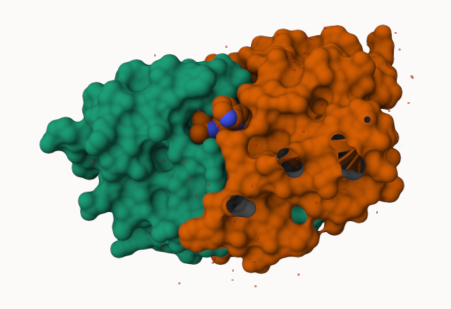
\includegraphics[keepaspectratio]{1HSG.png}}
\caption{My first image of HIV-Pr with surface display showing ligand
binding}
\end{figure}

A new clean image showing the catalytic ASP25 amino acids in both
chaings of the HIV-Pr dimer along with the inhibitor and all important
active site water.

\pandocbounded{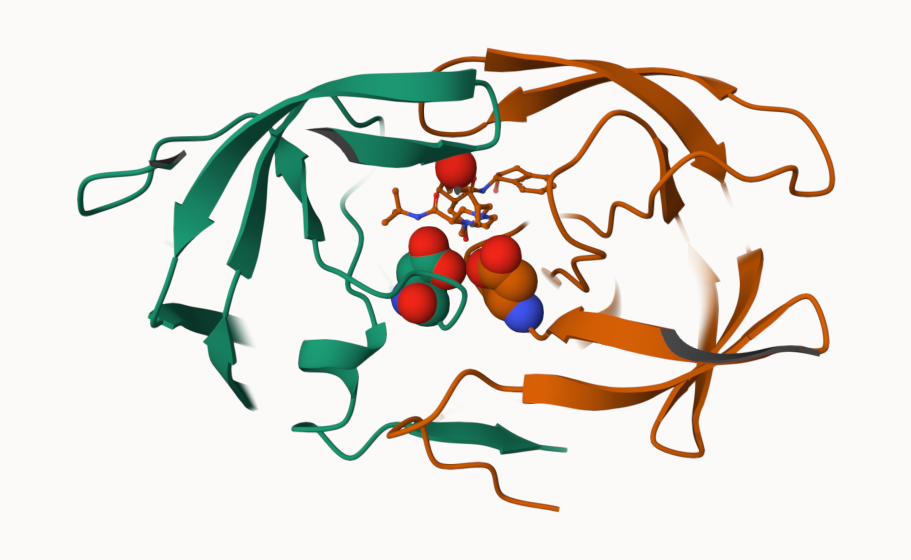
\includegraphics[keepaspectratio]{1HSG_2.png}}

\subsection{Bio3D package for structural
bioinformatics}\label{bio3d-package-for-structural-bioinformatics}

\begin{Shaded}
\begin{Highlighting}[]
\FunctionTok{library}\NormalTok{(bio3d)}

\NormalTok{pdb }\OtherTok{\textless{}{-}} \FunctionTok{read.pdb}\NormalTok{(}\StringTok{"1hsg"}\NormalTok{)}
\end{Highlighting}
\end{Shaded}

\begin{verbatim}
##   Note: Accessing on-line PDB file
\end{verbatim}

\begin{Shaded}
\begin{Highlighting}[]
\NormalTok{pdb}
\end{Highlighting}
\end{Shaded}

\begin{verbatim}
## 
##  Call:  read.pdb(file = "1hsg")
## 
##    Total Models#: 1
##      Total Atoms#: 1686,  XYZs#: 5058  Chains#: 2  (values: A B)
## 
##      Protein Atoms#: 1514  (residues/Calpha atoms#: 198)
##      Nucleic acid Atoms#: 0  (residues/phosphate atoms#: 0)
## 
##      Non-protein/nucleic Atoms#: 172  (residues: 128)
##      Non-protein/nucleic resid values: [ HOH (127), MK1 (1) ]
## 
##    Protein sequence:
##       PQITLWQRPLVTIKIGGQLKEALLDTGADDTVLEEMSLPGRWKPKMIGGIGGFIKVRQYD
##       QILIEICGHKAIGTVLVGPTPVNIIGRNLLTQIGCTLNFPQITLWQRPLVTIKIGGQLKE
##       ALLDTGADDTVLEEMSLPGRWKPKMIGGIGGFIKVRQYDQILIEICGHKAIGTVLVGPTP
##       VNIIGRNLLTQIGCTLNF
## 
## + attr: atom, xyz, seqres, helix, sheet,
##         calpha, remark, call
\end{verbatim}

\begin{Shaded}
\begin{Highlighting}[]
\CommentTok{\#head(pdb$atom)}
\end{Highlighting}
\end{Shaded}

\begin{Shaded}
\begin{Highlighting}[]
\CommentTok{\#install.packages("pak")}
\NormalTok{pak}\SpecialCharTok{::}\FunctionTok{pak}\NormalTok{(}\StringTok{"bioboot/bio3dview"}\NormalTok{)}
\end{Highlighting}
\end{Shaded}

\begin{verbatim}
## ! Using bundled GitHub PAT. Please add your own PAT using `gitcreds::gitcreds_set()`.
\end{verbatim}

\begin{verbatim}
## ℹ Loading metadata database✔ Loading metadata database ... done
##  
## ℹ No downloads are needed
## ✔ 1 pkg + 40 deps: kept 37 [7.7s]
\end{verbatim}

\begin{Shaded}
\begin{Highlighting}[]
\FunctionTok{library}\NormalTok{(bio3dview)}

\CommentTok{\#view.pdb(pdb)}
\end{Highlighting}
\end{Shaded}

\begin{Shaded}
\begin{Highlighting}[]
\CommentTok{\# Select the important ASP 25 residue}
\NormalTok{sele }\OtherTok{\textless{}{-}} \FunctionTok{atom.select}\NormalTok{(pdb, }\AttributeTok{resno=}\DecValTok{25}\NormalTok{)}

\CommentTok{\# and highlight them in spacefill representation}
\CommentTok{\#view.pdb(pdb, cols=c("navy","skyblue"), }
        \CommentTok{\# highlight = sele,}
        \CommentTok{\# highlight.style = "spacefill")}
\end{Highlighting}
\end{Shaded}

\subsection{Predicting functional motions of a single
structure}\label{predicting-functional-motions-of-a-single-structure}

Read an ADK structure from the PDB database:

\begin{Shaded}
\begin{Highlighting}[]
\NormalTok{adk }\OtherTok{\textless{}{-}} \FunctionTok{read.pdb}\NormalTok{(}\StringTok{"6s36"}\NormalTok{)}
\end{Highlighting}
\end{Shaded}

\begin{verbatim}
##   Note: Accessing on-line PDB file
##    PDB has ALT records, taking A only, rm.alt=TRUE
\end{verbatim}

\begin{Shaded}
\begin{Highlighting}[]
\NormalTok{adk}
\end{Highlighting}
\end{Shaded}

\begin{verbatim}
## 
##  Call:  read.pdb(file = "6s36")
## 
##    Total Models#: 1
##      Total Atoms#: 1898,  XYZs#: 5694  Chains#: 1  (values: A)
## 
##      Protein Atoms#: 1654  (residues/Calpha atoms#: 214)
##      Nucleic acid Atoms#: 0  (residues/phosphate atoms#: 0)
## 
##      Non-protein/nucleic Atoms#: 244  (residues: 244)
##      Non-protein/nucleic resid values: [ CL (3), HOH (238), MG (2), NA (1) ]
## 
##    Protein sequence:
##       MRIILLGAPGAGKGTQAQFIMEKYGIPQISTGDMLRAAVKSGSELGKQAKDIMDAGKLVT
##       DELVIALVKERIAQEDCRNGFLLDGFPRTIPQADAMKEAGINVDYVLEFDVPDELIVDKI
##       VGRRVHAPSGRVYHVKFNPPKVEGKDDVTGEELTTRKDDQEETVRKRLVEYHQMTAPLIG
##       YYSKEAEAGNTKYAKVDGTKPVAEVRADLEKILG
## 
## + attr: atom, xyz, seqres, helix, sheet,
##         calpha, remark, call
\end{verbatim}

\begin{Shaded}
\begin{Highlighting}[]
\NormalTok{m }\OtherTok{\textless{}{-}} \FunctionTok{nma}\NormalTok{(adk)}
\end{Highlighting}
\end{Shaded}

\begin{verbatim}
##  Building Hessian...     Done in 0.021 seconds.
##  Diagonalizing Hessian...    Done in 0.094 seconds.
\end{verbatim}

\begin{Shaded}
\begin{Highlighting}[]
\FunctionTok{plot}\NormalTok{(m)}
\end{Highlighting}
\end{Shaded}

\pandocbounded{
\includegraphics[keepaspectratio]{class10_structuralbioinformatics1_files/figure-latex/unnamed-chunk-15-1.pdf}}

Write out our results as a wee ttrajectory/movie of predicted motions:

\begin{Shaded}
\begin{Highlighting}[]
\FunctionTok{mktrj}\NormalTok{(m, }\AttributeTok{file=}\StringTok{"adk\_m7.pdb"}\NormalTok{)}
\end{Highlighting}
\end{Shaded}


\end{document}
